\section*{Malhas}

\begin{frame}[fragile]{Definição de sequência e de subsequência}

    \metroset{block=fill}
    \begin{block}{Definição}
        Uma \textbf{malha}, em geral, se refere a dois ou mais conjuntos de retas paralelas no plano, igualmente espaçadas, em ângulos específicos, ou às
        interseções de tais retas.
    \end{block}

    \vspace{0.3in}

    As malhas mais comuns são as quadradas, triangulares e hexagonais.

\end{frame}

\begin{frame}[fragile]{Malha quadrada}

    \begin{figure}[h]
        \centering

        \begin{tikz}
            \draw[thick] (1, 0) grid (13, 6);
        \end{tikz}

    \end{figure}

\end{frame}

\begin{frame}[fragile]{Malha triangular}

    \begin{figure}[h]
        \centering

        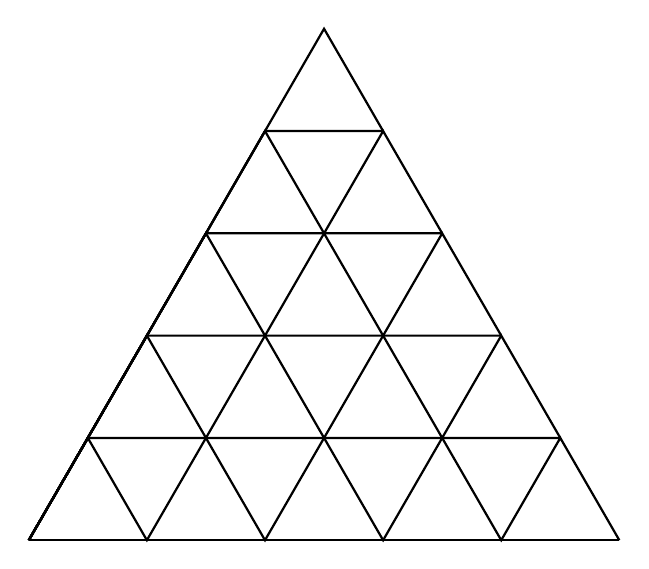
\begin{tikzpicture}
            \draw[thick] (1, 0) foreach \x in {1, ..., 5} { -- ++(60: 1.5) -- ++(300: 1.5) };
            \draw[thick] (1, 0) -- ++(60: 1.5) foreach \x in {1, ..., 4} { -- ++(60: 1.5) -- ++(300: 1.5) };
            \draw[thick] (1, 0) -- ++(60: 3) foreach \x in {1, ..., 3} { -- ++(60: 1.5) -- ++(300: 1.5) };
            \draw[thick] (1, 0) -- ++(60: 4.5) foreach \x in {1, ..., 2} { -- ++(60: 1.5) -- ++(300: 1.5) };
            \draw[thick] (1, 0) -- ++(60: 6) foreach \x in {1, ..., 1} { -- ++(60: 1.5) -- ++(300: 1.5) };

            \draw[thick] (1, 0) -- +(0: 7.5);
            \draw[thick] (1, 0) -- ++(60: 1.5) -- +(0: 6);
            \draw[thick] (1, 0) -- ++(60: 3) -- +(0: 4.5);
            \draw[thick] (1, 0) -- ++(60: 4.5) -- +(0: 3);
            \draw[thick] (1, 0) -- ++(60: 6) -- +(0: 1.5);
        \end{tikzpicture}

    \end{figure}

\end{frame}

\begin{frame}[fragile]{Malha hexagonal}

    \begin{figure}[h]
        \centering

        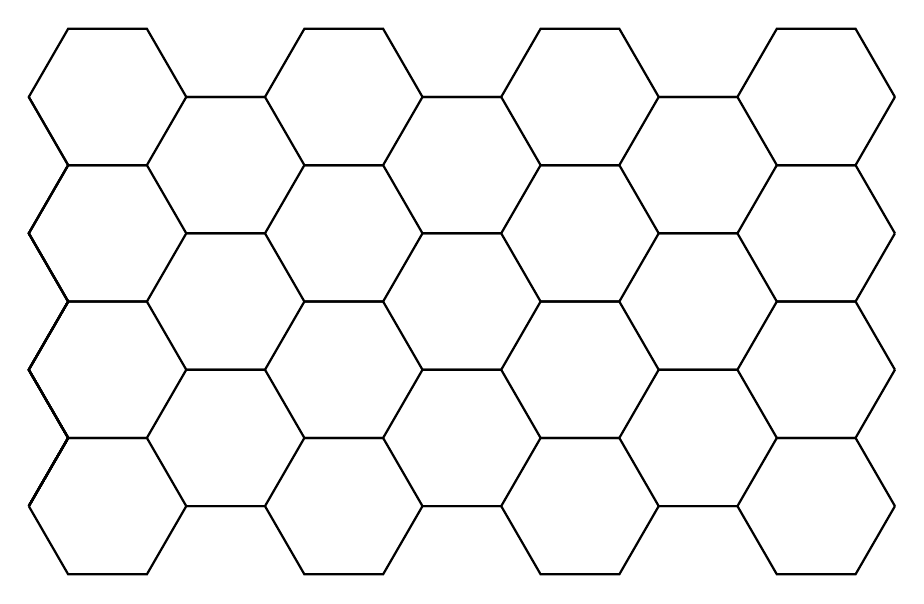
\begin{tikzpicture}
                \draw[thick] (1, 0) -- ++(300: 1) -- ++(0: 1) -- ++(60 : 1) -- ++(0: 1)
                    -- ++(300: 1) -- ++(0: 1) -- ++(60 : 1) -- ++(0: 1)
                    -- ++(300: 1) -- ++(0: 1) -- ++(60 : 1) -- ++(0: 1)
                    -- ++(300: 1) -- ++(0: 1) -- ++(60 : 1);

                \draw[thick] (1, 0) 
                    -- ++(60: 1) -- ++(0: 1) -- ++(300 : 1) -- ++(0: 1)
                    -- ++(60: 1) -- ++(0: 1) -- ++(300 : 1) -- ++(0: 1)
                    -- ++(60: 1) -- ++(0: 1) -- ++(300 : 1) -- ++(0: 1)
                    -- ++(60: 1) -- ++(0: 1) -- ++(300 : 1);

                \draw[thick] (1, 0) -- ++(60: 1) -- ++(120: 1) 
                    -- ++(300: 1) -- ++(0: 1) -- ++(60 : 1) -- ++(0: 1)
                    -- ++(300: 1) -- ++(0: 1) -- ++(60 : 1) -- ++(0: 1)
                    -- ++(300: 1) -- ++(0: 1) -- ++(60 : 1) -- ++(0: 1)
                    -- ++(300: 1) -- ++(0: 1) -- ++(60 : 1);

                \draw[thick] (1, 0) -- ++(60: 1) -- ++(120: 1) 
                    -- ++(60: 1) -- ++(0: 1) -- ++(300 : 1) -- ++(0: 1)
                    -- ++(60: 1) -- ++(0: 1) -- ++(300 : 1) -- ++(0: 1)
                    -- ++(60: 1) -- ++(0: 1) -- ++(300 : 1) -- ++(0: 1)
                    -- ++(60: 1) -- ++(0: 1) -- ++(300 : 1);

                \draw[thick] (1, 0) -- ++(60: 1) -- ++(120: 1) -- ++(60: 1) -- ++(120: 1) 
                    -- ++(300: 1) -- ++(0: 1) -- ++(60 : 1) -- ++(0: 1)
                    -- ++(300: 1) -- ++(0: 1) -- ++(60 : 1) -- ++(0: 1)
                    -- ++(300: 1) -- ++(0: 1) -- ++(60 : 1) -- ++(0: 1)
                    -- ++(300: 1) -- ++(0: 1) -- ++(60 : 1);

                \draw[thick] (1, 0) -- ++(60: 1) -- ++(120: 1) -- ++(60: 1) -- ++(120: 1) 
                    -- ++(60: 1) -- ++(0: 1) -- ++(300 : 1) -- ++(0: 1)
                    -- ++(60: 1) -- ++(0: 1) -- ++(300 : 1) -- ++(0: 1)
                    -- ++(60: 1) -- ++(0: 1) -- ++(300 : 1) -- ++(0: 1)
                    -- ++(60: 1) -- ++(0: 1) -- ++(300 : 1);

                \draw[thick] (1, 0) -- ++(60: 1) -- ++(120: 1) -- ++(60: 1) -- ++(120: 1) -- ++(60: 1) -- ++(120: 1) 
                    -- ++(300: 1) -- ++(0: 1) -- ++(60 : 1) -- ++(0: 1)
                    -- ++(300: 1) -- ++(0: 1) -- ++(60 : 1) -- ++(0: 1)
                    -- ++(300: 1) -- ++(0: 1) -- ++(60 : 1) -- ++(0: 1)
                    -- ++(300: 1) -- ++(0: 1) -- ++(60 : 1);

                \draw[thick] (1, 0) -- ++(60: 1) -- ++(120: 1) -- ++(60: 1) -- ++(120: 1) -- ++(60: 1) -- ++(120: 1) 
                    -- ++(60: 1) -- ++(0: 1) -- ++(300 : 1) -- ++(0: 1)
                    -- ++(60: 1) -- ++(0: 1) -- ++(300 : 1) -- ++(0: 1)
                    -- ++(60: 1) -- ++(0: 1) -- ++(300 : 1) -- ++(0: 1)
                    -- ++(60: 1) -- ++(0: 1) -- ++(300 : 1);


        \end{tikzpicture}

    \end{figure}

\end{frame}

\begin{frame}[fragile]{Malhas e sistemas de coordenadas}

    \begin{itemize}
        \item As malhas podem induzir um sistema de coordenadas e uma ordenação entre seus elementos básicos

        \item O sistema de coordenadas e a ordenação também podem ser arbitrários

        \item Conhecida a ordenação utilizada, duas questões se tornam relevantes:

        \begin{enumerate}[(a)]
            \item qual é a coordenada do $n$-ésimo ponto?
            \item as coordenadas dadas correspondem a qual ponto da ordenação?
        \end{enumerate}

        \item Responder estas perguntas dependem ou de uma observação atenta dos padrões gerados pelo sistema de coordenadas ou pela ordenação

        \item Em alguns casos é possível utilizar uma simulação para responder tais questões
    \end{itemize}

\end{frame}

\begin{frame}[fragile]{Exemplo: Zigue-zague em malhas quadradas}

    \begin{figure}[h]
        \centering

        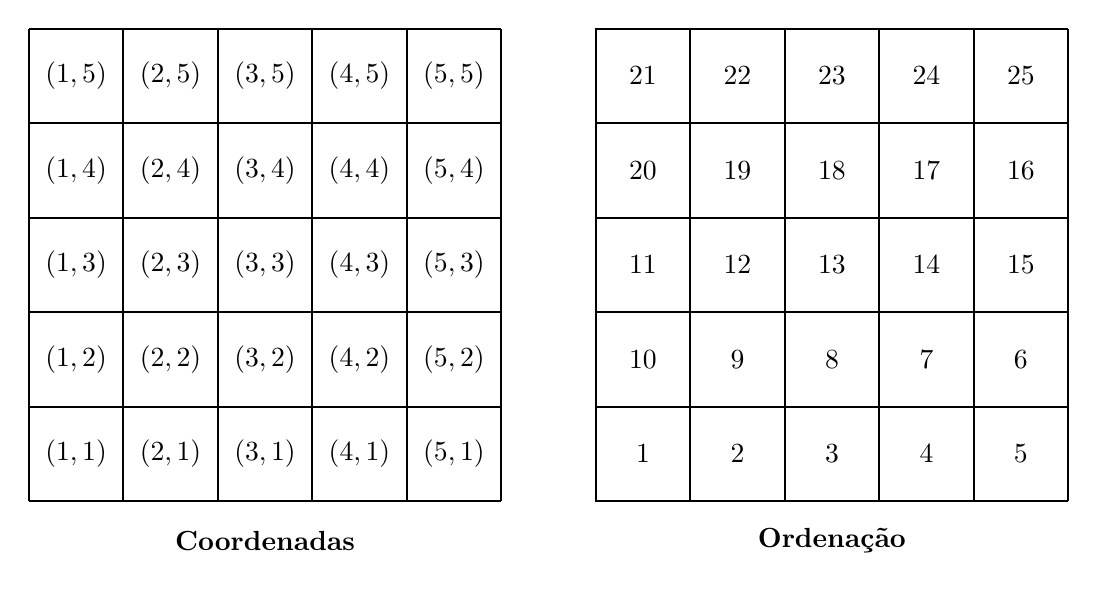
\begin{tikzpicture}
            \draw[thick,step = 1.2] (0, 0) grid (6, 6);
            \node at (3, -0.5) { \textbf{Coordenadas} };

            \draw[thick,step = 1.2] (7.19, 0) grid (13.2, 6);
            \node at (10.2, -0.5) { \textbf{Ordenação} };

            \foreach \x in {1, ..., 5 }
                \foreach \y in {1, ..., 5 }
                    \node at (-0.6 + \x*1.2, -0.6 + \y*1.2) { $(\x, \y)$ };
                
            \node at (7.8, 0.6) { $1$ };
            \node at (9.0, 0.6) { $2$ };
            \node at (10.2, 0.6) { $3$ };
            \node at (11.4, 0.6) { $4$ };
            \node at (12.6, 0.6) { $5$ };

            \node at (7.8, 1.8) { $10$ };
            \node at (9.0, 1.8) { $9$ };
            \node at (10.2, 1.8) { $8$ };
            \node at (11.4, 1.8) { $7$ };
            \node at (12.6, 1.8) { $6$ };

            \node at (7.8, 3) { $11$ };
            \node at (9.0, 3) { $12$ };
            \node at (10.2, 3) { $13$ };
            \node at (11.4, 3) { $14$ };
            \node at (12.6, 3) { $15$ };

            \node at (7.8, 4.2) { $20$ };
            \node at (9.0, 4.2) { $19$ };
            \node at (10.2, 4.2) { $18$ };
            \node at (11.4, 4.2) { $17$ };
            \node at (12.6, 4.2) { $16$ };

            \node at (7.8, 5.4) { $21$ };
            \node at (9.0, 5.4) { $22$ };
            \node at (10.2, 5.4) { $23$ };
            \node at (11.4, 5.4) { $24$ };
            \node at (12.6, 5.4) { $25$ };
        \end{tikzpicture}
    \end{figure}

\end{frame}

\begin{frame}[fragile]{Exemplo: Zigue-zague em malhas quadradas}

    \begin{itemize}
        \item Neste exemplo, o sistema de coordenadas é idêntico ao sistema cartesiano, onde as colunas são representadas pelas primeiras coordenadas do par e as linhas pelas segundas coordenadas

        \item A ordenação inicia no canto inferior esquerdo e avança até o fim da linha

        \item Ao subir para a próxima linha, a ordenação segue em sentido oposto, do final para o início da próxima linha, e assim por diante

        \item É possível simular esta ordenação por meio de um vetor de direção $\vec{u}$

        \item Inicialmente, $\vec{u} = (0, 1)$
    \end{itemize}

\end{frame}

\begin{frame}[fragile]{Exemplo: Zigue-zague em malhas quadradas}

    \begin{itemize}
        \item Sempre que os limites da malha forem atingidos, o vetor dever ser rotacionado em 180° 

        \item É possível, porém, determinar a posição $n$ referente à coordenada $(x, y)$ por meio da expressão
$$
    n = x + (y - 1)W,
$$
se $y$ é ímpar, e
$$
    n = (W - x + 1) + (y - 1)W ,
$$
se $y$ é par, onde $W$ é o número de colunas

    \end{itemize}

\end{frame}

\begin{frame}[fragile]{Exemplo: Zigue-zague em malhas quadradas}

    \begin{itemize}
        \item Também é possível determinar as coordenadas do $n$-ésimo ponto

        \item Este ponto estará na linha
$$
    y = \left\lfloor \frac{n - 1}{W} \right\rfloor + 1
$$
        \item Se $y$ é ímpar, a coluna será
$$
    x = [(n - 1)\ \mathrm{mod}\ W] + 1,
$$

        \item Se $y$ é par, então
$$
    x = W - [(n - 1)\ \mathrm{mod}\ W]
$$
    \end{itemize}

\end{frame}

\begin{frame}[fragile]{Implementação do zigue-zague em malhas quadradas}
    \inputsnippet{cpp}{5}{18}{codes/zigzag.cpp}
\end{frame}
